\documentclass[9pt,twocolumn,twoside]{../../styles/osajnl}
\usepackage{fancyvrb}
\journal{i524} 

\title{CoreOS}

\author[1, *]{Ribka Rufael}


\affil[1]{School of Informatics and Computing, Bloomington, IN 47408, U.S.A.}


\affil[*]{Corresponding authors: rrufael@umail.iu.edu HID: S17-IO-3016}

\dates{paper-001, February 25, 2017}

\ociscodes{CoreOS, Container, cloud, Linux}

% replace this with your url in github/gitlab
\doi{\url{https://github.com/cloudmesh/sp17-i524/blob/master/paper1/S17-IO-3016/report.pdf}}


\begin{abstract}
CoreOS is a minimal Linux operating system that allows application to
run on containers. CoreOS Linux is an operating system designed for
container  cluster frameworks. 
\newline
\end{abstract}

\setboolean{displaycopyright}{true}

\begin{document}

\maketitle

\section{Introduction}

CoreOS \cite{www-core} is a light weight linux operating system that
is designed to be used for container infrastructure. CoreOS allows
applications to run on containers so that there is abstraction layer
between applications and the operating system. The separation of
applications and operating system allows to avoid dependencies.
CoreOS can be run on clouds, virtual or physical servers. CoreOS
allows the ability for automatic software updates inorder to make sure
containers in cluster are secure and reliable. It also makes managing
large cluster environments easier. One of the differences between
CoreOS Linux and traditional Linux distribution is that, in the case
of traditional Linux distribution operating system, utilities and
software are puts together but in the case of CoreOS Linux only
operating system and utilities are bundled together. In CoreOS Linux
applications and software are run on containers. Figure 1 shows the
CoreOS Linux layout:


\begin{figure}[htbp]
\centering
\fbox{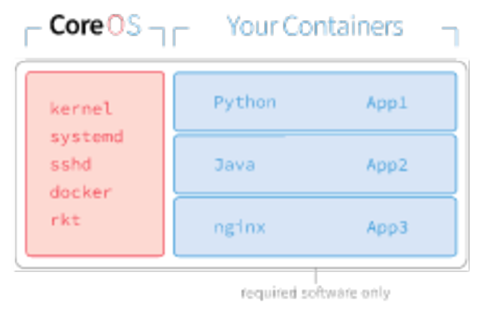
\includegraphics[width=\linewidth]{images/CoreOS}}
\caption{CoreOS container layout.  \cite{www-core} }
\label{fig:false-color}
\end{figure}

The company that provides CoreOS Linux also provides open source tools
like etcd, rkt and flannel. CoreOS also has commercial products
Kubernetes and CoreOS stack. In CoreOS linux service discovery is
achieved by etcd, applications are run on Docker and process
management is achieved by fleet.

Big data projects in science or business involve processing of large
amount of data.  These big data projects are hosted on bare metal
servers or on clouds. Big data projects in science and in business
sector can benefit from container frameworks that provide flexibility,
ease of deployment, adding or removing container clusters based on
demand. \cite{julian2016containers} Since CoreOS Linux is designed to
be used in container frameworks, it makes it one of the candidates to
be included into big data projects software stack that has container
cluster infrastructure.

\section{CoreOS Architecture and Installation}

CoreOS linux is a minimal operating system where the OS and utilities
are one unit and applications are run on containers. CoreOS has 9 disk
partitions. The disk partions are: 1) EFI-SYSTEM which contains the
bootloader and the partition type is VFAT. 2) BIOS-BOOT, ROOT-C and
the 7th partion these partions have no partion format and are reserved
for future use. 3) USR-A and USR- B are the active and passive
partions that container linux sits on. Only one of them can be active
at a time and partion type is EXT4 depending on which one is
active. 4) OEM has EXT4 as partition type and this is where OEM
platform related configurations like custom networking and running an
agent are stored. 5) OEM-CONFIG serves as an alternative place for an
OEM. 6) ROOT may have EXT4, BTRFS, or XFS as partion type and it is
used for keeping data which is persistent and this partion is
stateful. \cite{www-core}

CoreOS Linux comes bundled with etcd, Fleet and Docker. Service
discovery in CoreOS Linux is achieved by etcd. Key value store on etcd
is distributed and stored on all machines that run CoreOS Linux. This
service discovery capability makes it easy to add or remove
machines. There is a command line interface that comes preinstalled on
CoreOS linux called etcdctl that can be used to change and get key
value data from etcd using etcdctl set and etcdctl get
respectively. Another command that can be used for setting and reading key
value is curl.

Container management in CoreOS linux is made possible by Docker.  All
applications run on Docker. Containers can be launched using docker
run command line interface.

Fleet is the third component of CoreOS and it is used for management
of containers with Docker installed. Fleet is init system and fleetctl
command line interface can be used to check the status of containers,
start and stop containers.\cite{www-coreOSquickstart}

Based on the information in this book \cite{coreOSBook}, there is no package
manager for installing, upgrading, configuring softwares in CoreOS
. Softwares are installed as containers in CoreOS operating
system. Inorder to apply updates, CoreOS makes use of two root
partitions one is active and the other is passive.First the updates to
CoreOS are applied to passive partion and upon reboot all the updates
are applied to the active partition.

CoreOS can be installed on clouds from EC2, Rackspace, GCE or virtual
machines such as Vagrant, VMware, OpenStack or on physical servers
such as PXE, iPXE, ISO. \cite{www-coreOSquickstart}Based on the
information provided on CoreOS site \cite{www-coreOSvagrant}, CoreOS
container can be setup using Vagrant. Vagrant, virtual machine
manager, can be used to run CoreOS on a single machine with Windows,
OS X or Linux operating systems. It is recommened to have Vagrant
version 1.6.3 or latest. Virtual machines by VirtualBox or VMware are
both supported by Vagrant.

\section{Licensing}

CoreOS Container Linux is an open source operating system . It is
comprised of other programs and documents developed by other
individuals and companies. All original components that are part of
CoreOS Container Linux are licensed under Apache 2.0.  The latest
version of CoreOS Container Linux is 1325.1.0. \cite{www-core}


\section{Performance}

In a study done by Purdue University \cite{julian2016containers} ,
performance tests between CoreOS 899.5.0 on Docker and Red Hat
Enterprise Linux 6.5 were performed. In their study, the tests were
run on 24-core AMD Opteron systems, with 2.1 GHz processors, 48 GB
memory and 10Gbps Ethernet connection.  For HPL performance tests the
results were “The native RHEL 6.5 system showed an average performance
of 7.839 GFLOPS, versus 7.811 GFLOPS in a containerized environment
(approximately a 0.4\% slowdown). ” The netwrok throughput iperf was
used and the results were: “final upload throughput was 8.43 Gbps
under Docker (versus 8.26 Gbps in RHEL 6.5), with a download
throughput of 9.37 Gbps (versus 9.38 Gbps in RHEL 6.5). ” Network File
System throughput was done using iozone and results are shown in
Figure 2:

\begin{figure}[htbp]
\centering
\fbox{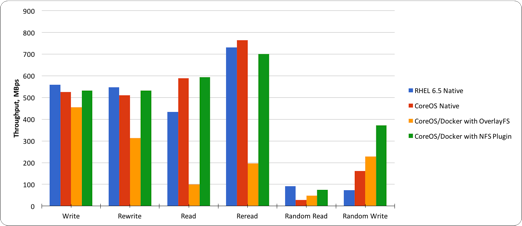
\includegraphics[width=\linewidth]{images/File-server-throughput}}
\caption{File Server throughput. \cite{julian2016containers} }
\label{fig:false-color}
\end{figure}

In another study done in Institute of Informatics – Federal University
of Rio Grande do Sul \cite{2016NFVSolutions}, performance analysis of
ClickOS, CoreOS and OS\textsuperscript{v} was performed. “NFV is a new
networking paradigm where functions (e.g., firewalls, DNS, IDS),
traditionally performed by dedicated physical devices, are virtualized
and deployed on commodity hardware. ” In their paper comarision of
ClickOS, CoreOS and OS\textsuperscript{v} as NFV based tools was
performed. They comapred boot time, response time and memory
consumption for the three virtualization technologies. As per their
evaluation result, ClickOS has the lowest boot time and response time
followed by CoreOS and with regards to memory cosumption, CoreOS has
the smallest memory usage followed by ClickOS. Based on the result
OS\textsuperscript{v} has the slowest boot time and response time as
compared to CoreOS and ClickOS. Also for memory consumption,
OS\textsuperscript{v} has the highest cosumption as compared to the
other two technologies used.

\section{Use Cases}

In this section use cases from big data and other areas where CoreOS
Linux is used are discused.

\subsection{Use Cases  for Big Data}

According to \cite{meyer2008metagenomics} , Metagenomics RAST
server(MG-RAST) is free access portal that can be used by researchers
for accessing and analyzing metagenomics data. “Random community
genomes (metagenomes) are now commonly used to study microbes in
different environments. ” As described on \cite{wilke2016mg}, CoreOS and
fleet are used on MG-RAST container application servers. Researchers
can input data into MG-RAST portal through script, web site or REST
API.

\subsection{Other Use Cases}
According to the paper \cite{2SPRA}, CoreOS container linux on Amazon
EC2 cloud was used to implement the project Two-stage Stochastic
Programming Resource Allocator (2SPRA). The language used to implement
was Python. In this project,they try to address the problem that exist
in most datacenters of over provisioning resources in order to achieve
performance service level objective. 2SPRA is a resource allocation
scheme and it is able to optimize resource allocation for
containerized web services based on varying workloads. 2SPRA analyses
the relationship between change in workload, resource allocation and
response latency inorder to calculate the the number of containers
needed. In this experimental work, CoreOS was used inorder to simulate
real word scenarios of n tier application servers running on
containers. The test architecture has client Java based emulator which
creates multiple user sessions at the same time, web hosting platform
with where RUBis benchmark is installed on Virtual machine with CoreOS
version stable r717.3.0 and the third component is 2SPRA implemented
in Python running on Virtual machine.


\section{Educational material} 

CoreOS website \cite{www-coreOSquickstart} has detailed documentation
and materials for anyone who is interested in setting up CoreOS
Container linux on clouds, virtual or physical servers.  Users who are
interested can contribute to the CoreOS open source projects through
github \cite {www-coregit}.

This book \cite{coreOSBook} also has information about CoreOS overview
and its installation.

\section{Conclusion} 
CoreOS Linux is a light weight Linux based operating system that is
designed for containers. It provides abstraction by separating the
operating system from application and softwares. Operating system
updates to CoreOS are automatic without a need for user
interaction. CoreOS can be installed on clouds from EC2, Rackspace,
GCE or virtual machines such as Vagrant, VMware, OpenStack or on
physical servers such as PXE, iPXE, ISO.  

CoreOS Linux makes applications and microservices running on
containers secure, easy to deploy and portable. Big data projects can
leverage these benefits that comes with CoreOS Linux by adding it to
their infrastructure.

As previous performance results has shown \cite{2016NFVSolutions},
CoreOS Linux has the lowest memory usage compared to other
operating systems namely ClickOS and OS\textsuperscript{v}.


\section*{Acknowledgements}
The author would like to thank Professor Gregor von Laszewski and
associate instructors for their help and guidance.



% Bibliography

\bibliography{references}
 

\newpage

\appendix



\end{document}
